\documentclass[a4paper]{report}
\usepackage[italian]{babel}
\usepackage[utf8]{inputenc}
\usepackage{hyperref, graphicx, colortbl, gensymb}
\hypersetup{colorlinks=true, urlcolor=blue, linkcolor=black}
\title{Controllo di un motore brushless}
\author{Stefano Cattonar}
\date{Giugno 2019}

\begin{document}

\maketitle
\tableofcontents

\section*{Introduzione}
La corrente elettrica passa in un filo di rame che avvolge a spirale un pezzo di ferro dolce chiamato
rotore. Questo avvolgimento, crea un campo elettromagnetico al passaggio di corrente. Questo campo elettromagnetico è immerso in un altro campo magnetico creato dallo statore, che nel caso più semplice è costituito da una o più calamite, o elettrocalamite. Il rotore per induzione elettromagnetica inizia a girare, in
quanto il "nord" del campo magnetico del rotore è attratto dal
"sud" del campo magnetico dello statore e viceversa. Ogni
mezzo giro la polarità viene invertita, in modo da dare
continuità alla rotazione nel secondo mezzo giro ...e così via.

Durante la trasformazione, una modesta parte dell'energia
viene dispersa in calore per l'effetto Joule. Il motore elettrico a seconda della sua tensione di
alimentazione, e del suo comportamento, può essere un motore asincrono, motore sincrono, o un
motore in corrente continua.


    Formula della coppia in un motore elettrico:
    \newline
    \begin{center}\LARGE{
    \framebox{$T={V*w*k\over{r}}*k.$}
    }
    \end{center}
    
    
        T = Momento Torcente

        V = Voltaggio

        w = Velocità di rotazione

        k = Costante del motore

        R = Resistenza

    \newpage
    Per il corso di laboratorio ciberfisico abbiamo dovuto implementare il software di gestione di un motore brushless attraverso la programmazione a basso livello di una board della \href{https://www.st.com/}{STMicroelectronics}.Nel nostro caso una ST-NucleoF401RE.
    \begin{figure}[h]
    \centering
    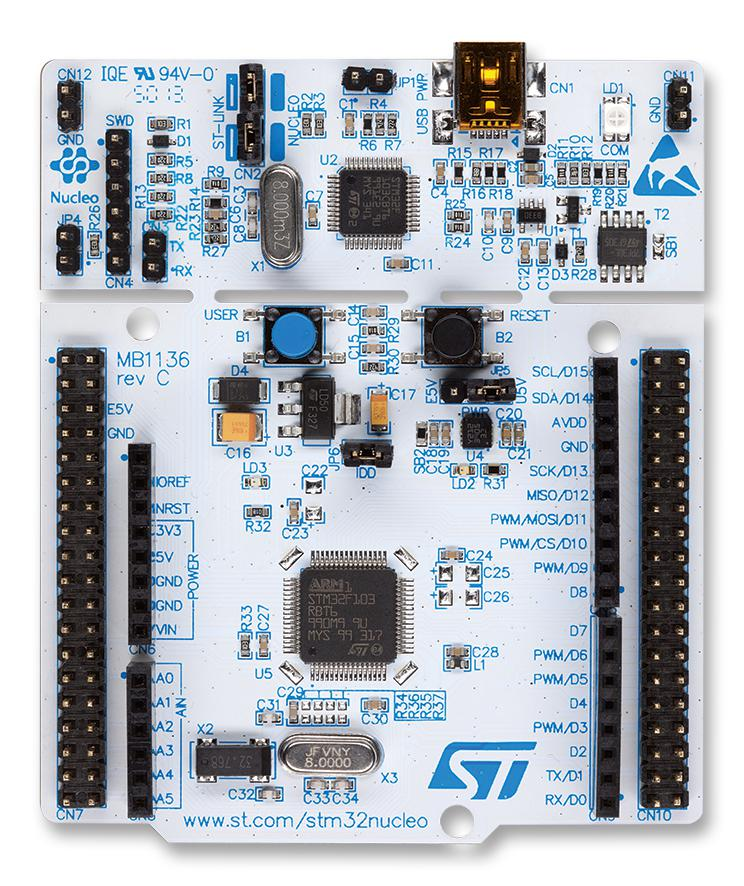
\includegraphics[scale=0.2, keepaspectratio=true]{nucleo}
    \end{figure}

    \newpage
\chapter{Teoria}.
\section{Algoritmo Six-Step Commutation}


    \subsection{Descrizione dell'algoritmo}

        L'algoritmo {``}\textit{Six-Step Commutation}{"} è necessario per la corretta rotazione del motore.
        Come dice la parola inglese \textbf{commutation} presente nel nome dell'algoritmo, si tratta di commutare, cioè di eseguire la cummutazione dei tre circuiti elettrici presenti.

    \subsection{Implementazione dell'algoritmo}
        Per poter implementare l'algoritmo bisogna conoscere le seguenti cose:
        \begin{itemize}
            \item Conoscere il numero di poli magnetici del proprio motore
            \item Conoscere il numero di spire del proprio motore
        \end{itemize}
        Dopodiché si può creare la tabella di commutazione.
        Nel prossimo capitolo mostrerò l'implementazione per il nostro motore.

\chapter{Pratica}
\section{Tabella di Commut.azione}
    Il nostro brushless ha 2 poli magnetici come si può vedere dall'immagine sottostante:
    \begin{figure}[h]
        \centering
        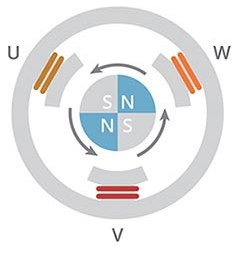
\includegraphics[scale=0.7, keepaspectratio=true]{poli}
    \end{figure}

    La nostra tabella di commutazione quindi si presenta così:
    \begin{table}[htbp]
        \centering
            \begin{tabular}{|c|c|c|}
                \hline
                U & V & W \\\hline
                + & - & off\\ \hline
                - & off & - \\ \hline
                off & + & - \\ \hline
                - & + & off \\ \hline
                - & off & + \\ \hline
                off & - & + \\ \hline
            \end{tabular}
            \label{tab:tabella di commutazione}
    \end{table}

    Creata la tabella di commutazione è necessario capire il numero di volte in cui le sei fasi si ripetono in un giro completo.
    \begin{figure}[htbp]
    \centering
    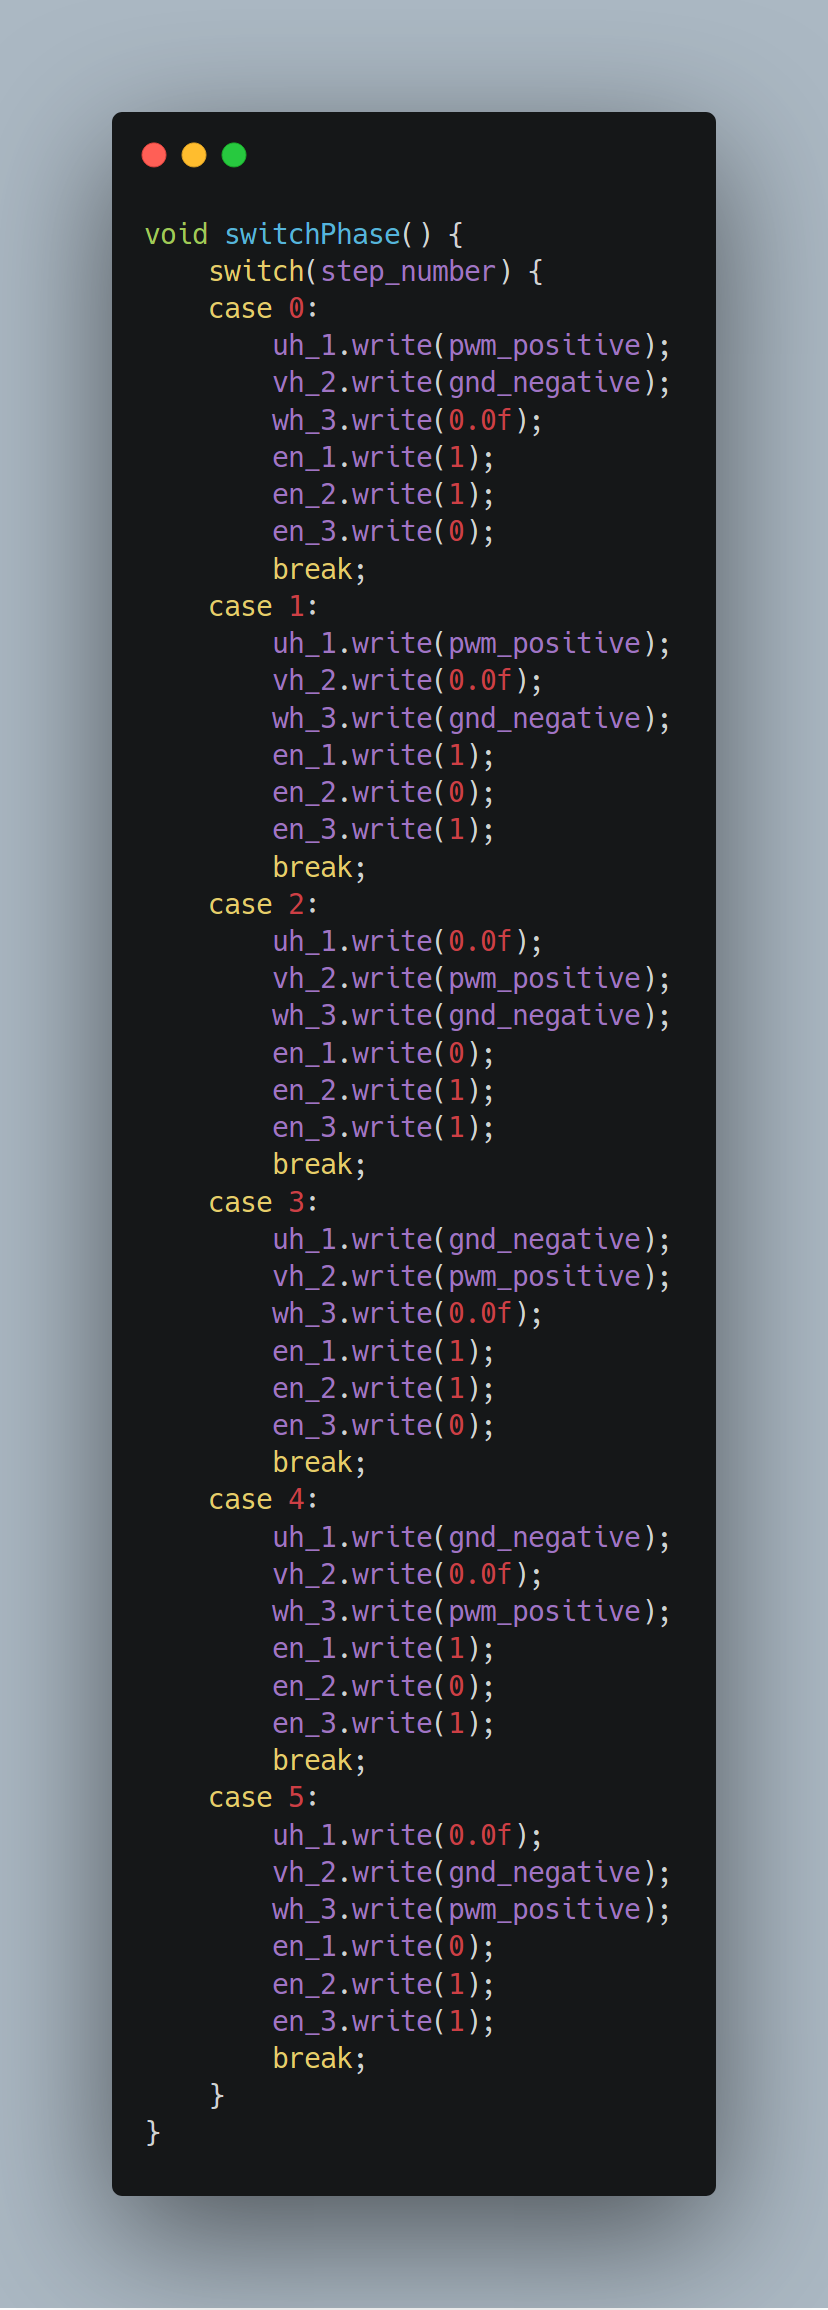
\includegraphics[scale=0.1,keepaspectratio=true]{table}
    \caption{Implementazione del codice della tabella}    
    \end{figure}

    Nel nostro caso le sei fasi permettono di fare solo 51\degree {~}di rotazione, quindi: $360/51=7.$
    Visto che il totale delle fasi fa 51\degree circa ogni fase equivale a $51/6=8,5\degree$.
    
    \begin{figure}[htbp]
    \centering
    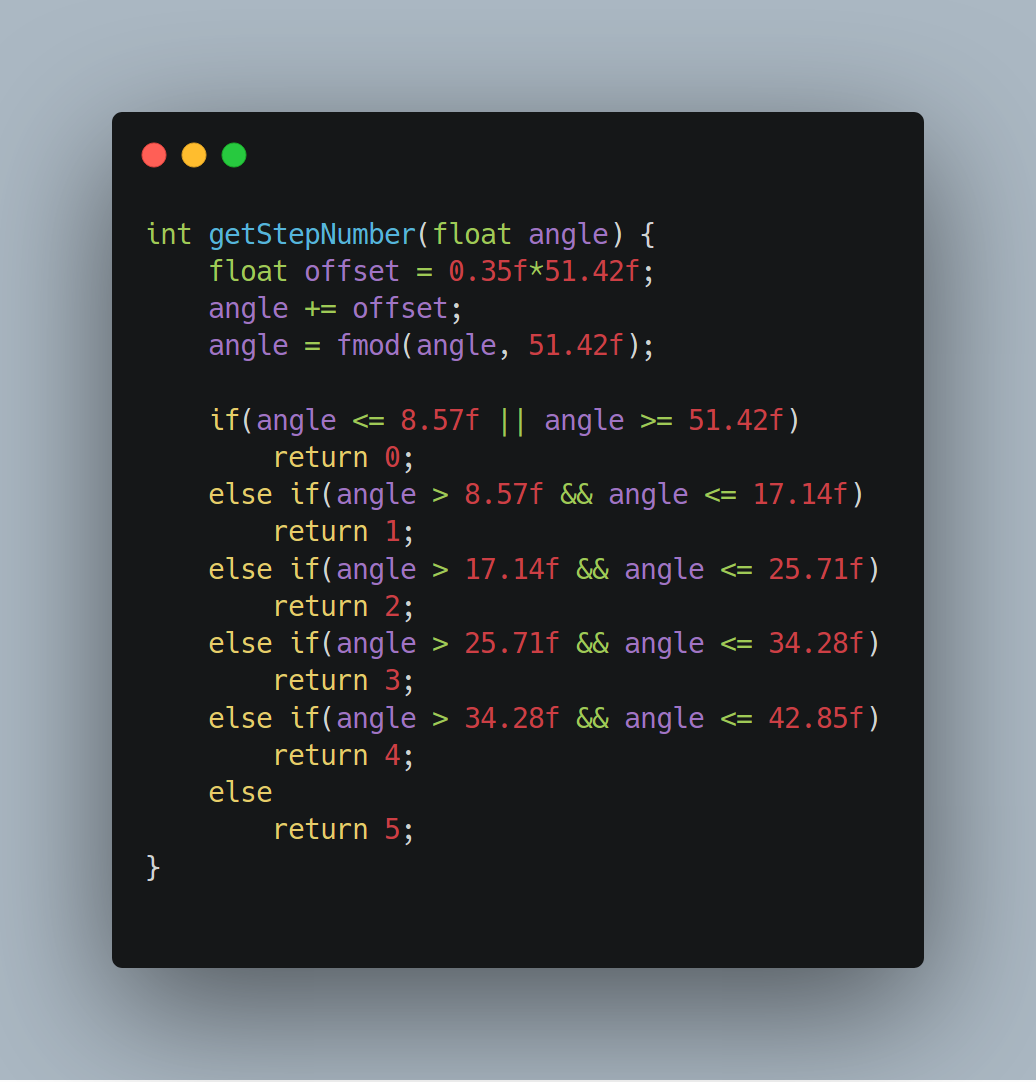
\includegraphics[scale=0.3,keepaspectratio=true]{step}
    \caption{Implementazione dell'algoritmo}    
    \end{figure}

Una volta caricato questo codice C++ sulla board(insieme ad altro codice che sarà lasciato al lettore), il nostro motore è in grado di produrre una rotazione continua e quindi una coppia costante in una direzione.



%Work in progress... o forse no.
    

\end{document}
